%==============================================================================
% TEMPLATE LAPORAN AKHIR PROYEK PENGGANTI UAS
% Mata Kuliah Kecerdasan Buatan | Teknik Komputer - Universitas Indonesia
% Semester Genap 2025/2026
%
% Cara pakai:
%   1. Ganti seluruh teks yang ada di dalam [...] atau \TODO{...}.
%   2. Hapus blok "petunjuk" (yang ditandai dengan environment "petunjuk")
%      setelah subbab terkait selesai diisi.
%   3. Kompilasi dengan XeLaTeX (rekomendasi):
%        xelatex template-laporan-akhir.tex
%        xelatex template-laporan-akhir.tex    % run ke-2 untuk DaftarIsi/refs
%   4. Sitasi pakai BibTeX gaya IEEE (file referensi.bib).
%==============================================================================

\documentclass[11pt,a4paper,oneside]{report}

%------ Bahasa & Font --------------------------------------------------------
\usepackage{fontspec}
\setmainfont{Times New Roman}
\setmonofont{Consolas}[Scale=0.92]

%------ Geometri & Spasi -----------------------------------------------------
\usepackage[a4paper,margin=2.5cm]{geometry}
\usepackage{setspace}
\onehalfspacing
\setlength{\parskip}{0.5em}

%------ Paket Pendukung ------------------------------------------------------
\usepackage{graphicx}
\usepackage{amsmath,amssymb,amsfonts}
\usepackage{booktabs}
\usepackage{array}
\usepackage{tabularx}
\usepackage{longtable}
\usepackage{enumitem}
\usepackage{xcolor}
\usepackage{listings}
\usepackage{hyperref}
\usepackage{titlesec}
\usepackage{tcolorbox}
\usepackage{caption}
\usepackage[backend=biber,style=ieee]{biblatex}

%------ Penyesuaian Bahasa Indonesia (manual, tanpa babel) -------------------
\renewcommand{\chaptername}{BAB}
\renewcommand{\contentsname}{DAFTAR ISI}
\renewcommand{\listfigurename}{DAFTAR GAMBAR}
\renewcommand{\listtablename}{DAFTAR TABEL}
\renewcommand{\bibname}{DAFTAR PUSTAKA}
\renewcommand{\appendixname}{LAMPIRAN}
\renewcommand{\figurename}{Gambar}
\renewcommand{\tablename}{Tabel}

%------ Format Bab (BAB I, BAB II, ...) --------------------------------------
\titleformat{\chapter}[display]
  {\normalfont\Large\bfseries\centering}
  {\chaptername\ \thechapter}{12pt}{\Large}
\titlespacing*{\chapter}{0pt}{-20pt}{20pt}

%------ Hyperref -------------------------------------------------------------
\hypersetup{
  colorlinks=true,
  linkcolor=black,
  urlcolor=blue,
  citecolor=black,
  pdftitle={Laporan Akhir Proyek - MK Kecerdasan Buatan},
  pdfauthor={Kelompok [KodeKelompok]}
}

%------ Box Petunjuk Pengisian (HAPUS setelah subbab terisi) ----------------
\newtcolorbox{petunjuk}{
  colback=yellow!10,
  colframe=orange!60!black,
  boxrule=0.5pt,
  arc=2pt,
  left=6pt,right=6pt,top=4pt,bottom=4pt,
  fontupper=\small\itshape
}

%------ Listing untuk JSON ---------------------------------------------------
\lstdefinelanguage{json}{
  basicstyle=\ttfamily\footnotesize,
  showstringspaces=false,
  breaklines=true,
  frame=single,
  rulecolor=\color{gray!50},
  string=[s]{"}{"},
  stringstyle=\color{blue!60!black},
  comment=[l]{//},
  commentstyle=\color{green!50!black}
}

%------ Bibliography (siapkan referensi.bib di folder yang sama) -------------
\addbibresource{referensi.bib}

%==============================================================================
\begin{document}

%==============================================================================
% HALAMAN SAMPUL
%==============================================================================
\begin{titlepage}
\centering
\vspace*{1cm}

{\Large\bfseries LAPORAN AKHIR \par}
{\large PROYEK PENGGANTI UAS \par}
\vspace{0.3cm}
{\large Mata Kuliah Kecerdasan Buatan \par}
{\large Semester Genap 2025/2026 \par}

\vspace{2cm}

% Logo opsional
% \includegraphics[width=0.25\textwidth]{logo-ui.png}

\vspace{1.5cm}

{\LARGE\bfseries [JUDUL PROYEK YANG DESKRIPTIF] \par}
\vspace{0.5cm}
{\large Subjudul: Topik / Model AI yang Digunakan \par}

\vspace{2.5cm}

{\large Disusun oleh: \par}
\vspace{0.5cm}
\begin{tabular}{rl}
{Benedict Aurelius} & NPM. 2306213174 \\
{Deandro Najwan Ahmad Syahbanna}& NPM. 2306213174 \\
{Nelson Laurensius} & NPM. 2306161845 \\
{Wesley Frederick Oh} & NPM. 2306202763 \\
\end{tabular}

\vspace{2cm}

{\large Dosen Pengampu: \par}
{\large [Nama Dosen Pengampu] \par}

\vfill

{\large DEPARTEMEN TEKNIK KOMPUTER \par}
{\large FAKULTAS TEKNIK \par}
{\large UNIVERSITAS INDONESIA \par}
{\large [BULAN] 2026 \par}
\end{titlepage}

%==============================================================================
% LEMBAR PERNYATAAN ORISINALITAS
%==============================================================================
\chapter*{LEMBAR PERNYATAAN ORISINALITAS}
\addcontentsline{toc}{chapter}{Lembar Pernyataan Orisinalitas}

Kami yang bertandatangan di bawah ini menyatakan bahwa laporan ini, beserta seluruh isinya (termasuk Sub-bab IV.x masing-masing anggota dan berkas \texttt{metadata.json} yang merupakan bagian tidak terpisahkan), adalah hasil karya kelompok kami sendiri. Setiap kutipan, kode, atau gambar yang berasal dari sumber lain telah disitasi dengan benar. Penggunaan AI \textit{assistant} telah dideklarasikan secara jujur pada Sub-bab IV.x.2.

\vspace{1.5cm}

\noindent
\begin{tabular}{p{0.45\textwidth}p{0.45\textwidth}}
\centering [Nama Anggota 1] & \centering [Nama Anggota 2] \tabularnewline
\centering NPM. [xxxxxxxxxx] & \centering NPM. [xxxxxxxxxx] \tabularnewline
\vspace{1.5cm} & \vspace{1.5cm} \tabularnewline
\centering (\hspace{4cm}) & \centering (\hspace{4cm}) \tabularnewline
\end{tabular}

\vspace{1cm}

\noindent
\begin{tabular}{p{0.45\textwidth}p{0.45\textwidth}}
\centering [Nama Anggota 3] & \centering [Nama Anggota 4 - jika ada] \tabularnewline
\centering NPM. [xxxxxxxxxx] & \centering NPM. [xxxxxxxxxx] \tabularnewline
\vspace{1.5cm} & \vspace{1.5cm} \tabularnewline
\centering (\hspace{4cm}) & \centering (\hspace{4cm}) \tabularnewline
\end{tabular}

%==============================================================================
% DAFTAR ISI, GAMBAR, TABEL
%==============================================================================
\tableofcontents
\listoffigures
\listoftables

%==============================================================================
% ABSTRAK
%==============================================================================
\chapter*{ABSTRAK}
\addcontentsline{toc}{chapter}{Abstrak}

\begin{petunjuk}
Maksimum 250 kata. Tulis dalam satu paragraf utuh. Cakupi: konteks masalah singkat, pendekatan AI yang digunakan, dataset, metrik utama, dan hasil kuantitatif terpenting (angka konkret). Hindari kalimat klise seperti ``proyek ini bertujuan untuk mengeksplorasi\ldots''. Mulai langsung dengan substansi.
\end{petunjuk}

[ISI ABSTRAK DI SINI]

\vspace{1em}
\noindent\textbf{Kata kunci:} [3--5 kata kunci dipisahkan koma]

%==============================================================================
% BAB I - PENDAHULUAN & DEFINISI MASALAH
%==============================================================================
\chapter{PENDAHULUAN \& DEFINISI MASALAH}
\label{bab:pendahuluan}

\section{Topik yang Dipilih}
\begin{petunjuk}
Sebutkan 1 dari 5 topik yang disediakan tim pengajar. Tuliskan alasan pemilihan dalam 1--2 paragraf: keterkaitan dengan keahlian tim, ketersediaan data, urgensi domain. Tidak perlu panjang.
\end{petunjuk}

[ISI DI SINI]

\section{Rumusan Masalah}
\begin{petunjuk}
1--3 pertanyaan riset yang jelas dan terukur. Format: \textit{``Bagaimana / Sejauh mana / Apakah\ldots?''}. Setiap pertanyaan harus dapat dijawab oleh hasil eksperimen di Bab III dan disimpulkan di Bab V.
\end{petunjuk}

\begin{enumerate}[label=RM\arabic*.,leftmargin=*]
    \item {[Rumusan masalah pertama]}
    \item {[Rumusan masalah kedua (jika ada)]}
    \item {[Rumusan masalah ketiga (jika ada)]}
\end{enumerate}

\section{Tujuan Proyek}
\begin{petunjuk}
2--4 tujuan terukur. Gunakan kata kerja aktif: \textit{menerapkan, mengevaluasi, membandingkan, menganalisis}. Setiap tujuan harus terhubung ke salah satu rumusan masalah.
\end{petunjuk}

\begin{enumerate}[label=T\arabic*.,leftmargin=*]
    \item {[Tujuan pertama]}
    \item {[Tujuan kedua]}
\end{enumerate}

\section{Ruang Lingkup \& Batasan}
\begin{petunjuk}
Sebutkan domain data, varian model, dan metrik yang dievaluasi. Yang sama pentingnya: \textbf{sebutkan secara eksplisit hal-hal yang TIDAK dikerjakan} (mis. ``tidak melakukan tuning arsitektur layer-by-layer'', ``tidak mengevaluasi pada data \textit{out-of-distribution}''). Hal ini menjadi acuan saat sesi ujian lisan.
\end{petunjuk}

[ISI DI SINI]

%==============================================================================
% BAB II - PENDEKATAN AI
%==============================================================================
\chapter{PENDEKATAN AI}
\label{bab:pendekatan}

\section{Tinjauan Pustaka (\textit{Related Work})}
\begin{petunjuk}
Sajikan 3--5 referensi terpenting dalam bentuk tabel ringkas. Akhiri dengan satu kalimat yang menjelaskan \textbf{posisi proyek ini terhadap literatur}: apa yang baru / berbeda / belum dilakukan oleh penulis lain.
\end{petunjuk}

\begin{table}[h!]
\centering
\caption{Ringkasan tinjauan pustaka}
\label{tab:related-work}
\begin{tabularx}{\textwidth}{lXXXX}
\toprule
\textbf{Penulis (Th.)} & \textbf{Metode} & \textbf{Dataset} & \textbf{Hasil} & \textbf{Keterbatasan} \\
\midrule
{[Penulis]} \cite{ref1} & [Metode] & [Dataset] & [Metrik\&Hasil] & [Keterbatasan] \\
{[Penulis]} \cite{ref2} & [Metode] & [Dataset] & [Metrik\&Hasil] & [Keterbatasan] \\
{[Penulis]} \cite{ref3} & [Metode] & [Dataset] & [Metrik\&Hasil] & [Keterbatasan] \\
\bottomrule
\end{tabularx}
\end{table}

[Paragraf posisi proyek terhadap literatur.]

\section{Landasan Teori Model yang Dipilih}
\begin{petunjuk}
Jelaskan arsitektur model yang dipilih. Sertakan minimal 1 persamaan matematis kunci sesuai topik (CNN: operasi konvolusi; RNN/LSTM/GRU: persamaan \textit{gate}; GNN: \textit{message passing}; Transformer: \textit{scaled dot-product attention}; RL: persamaan Bellman / \textit{policy gradient}). Sertakan diagram arsitektur (boleh dari paper, beri sitasi).
\end{petunjuk}

[Penjelasan komponen utama arsitektur.]

\begin{equation}
\label{eq:persamaan-utama}
[\text{persamaan matematis kunci di sini}]
\end{equation}

dengan $[variabel]$ adalah \ldots, $[variabel]$ adalah \ldots, dan $[variabel]$ adalah \ldots.

\begin{figure}[h!]
\centering
% \includegraphics[width=0.75\textwidth]{gambar/arsitektur.png}
\fbox{\parbox[c][4cm][c]{0.75\textwidth}{\centering [Diagram arsitektur model]}}
\caption{Arsitektur [nama model] (Sumber: \cite{ref1})}
\label{fig:arsitektur}
\end{figure}

\section{Justifikasi Ilmiah Pemilihan Pendekatan AI}
\begin{petunjuk}
\textbf{Wajib.} Bagian ini akan menjadi sumber utama pertanyaan ujian lisan tipe konseptual. Jelaskan:
(1) mengapa arsitektur ini, bukan alternatif yang relevan (mis. mengapa Transformer bukan LSTM untuk kasus ini);
(2) \textit{tradeoff} yang dipertimbangkan (akurasi vs kecepatan vs ukuran model vs kebutuhan data);
(3) konteks domain yang membuat pilihan ini superior.
\end{petunjuk}

[ISI DI SINI - tulis dengan presisi.]

\section{\textit{Block Diagram} Sistem End-to-End}
\begin{petunjuk}
Diagram alur lengkap: data → preprocessing → model → loss/reward → metrik → output.
\end{petunjuk}

\begin{figure}[h!]
\centering
\fbox{\parbox[c][4cm][c]{0.85\textwidth}{\centering [Block diagram sistem end-to-end]}}
\caption{Block diagram sistem yang diusulkan}
\label{fig:block-diagram}
\end{figure}

\section{\textit{Flowchart} Program}
\begin{petunjuk}
Alur runtime program (\textit{training} \& \textit{inference}) dalam notasi flowchart standar.
\end{petunjuk}

\begin{figure}[h!]
\centering
\fbox{\parbox[c][4cm][c]{0.85\textwidth}{\centering [Flowchart program]}}
\caption{Flowchart program training dan inference}
\label{fig:flowchart}
\end{figure}

%==============================================================================
% BAB III - IMPLEMENTASI & HASIL EKSPERIMEN
%==============================================================================
\chapter{IMPLEMENTASI \& HASIL EKSPERIMEN}
\label{bab:implementasi}

\section{Dataset \& Pra-pemrosesan}
\begin{petunjuk}
Sumber, lisensi, ukuran, jumlah kelas, distribusi. Sertakan contoh sampel (minimal 3). Tuliskan \textit{train/validation/test split} (ratio + jumlah absolut). \textbf{Cantumkan random seed} yang digunakan.
\end{petunjuk}

\begin{sloppypar}
Pada eksperimen ini, dataset yang digunakan adalah \textit{National Tsing Hua University Driver Drowsiness Detection} (NTHU-DDD) \textit{Multi-Class} dari Kaggle. Dataset ini memiliki total tepat 66.521 gambar yang terbagi ke dalam 4 kelas objek perilaku pengemudi dan 1 kelas \textit{background}. Distribusi gambar untuk masing-masing kelas objek adalah: \texttt{notdrowsy} (30.491), \texttt{sleepyCombination} (17.756), \texttt{slowBlinkWithNodding} (9.412), dan \texttt{yawning} (8.862).  

Gambar \ref{fig:contoh-dataset} memperlihatkan tiga contoh sampel citra dari kelas yang berbeda yang digunakan dalam \textit{training}.

\begin{figure}[!ht]
\centering

\begin{minipage}{0.28\textwidth}
\centering
\fbox{
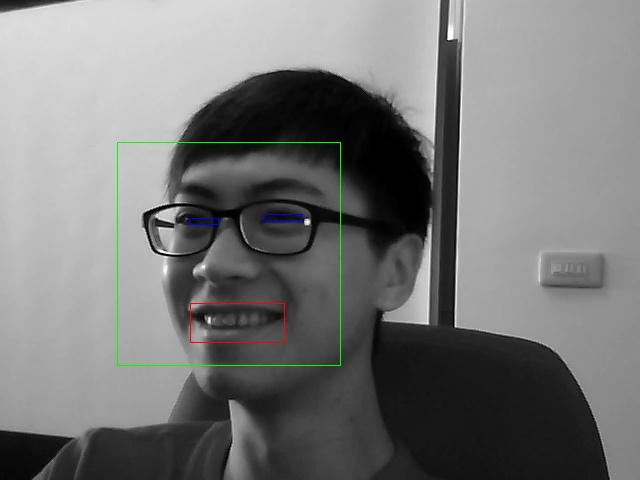
\includegraphics[
    width=0.95\linewidth,
    height=3cm,
    keepaspectratio
    ]{images/001_glasses_nonsleepyCombination_1014_notdrowsy.jpg}
}
\caption*{a) \texttt{notdrowsy}}
\end{minipage}
\hfill
\begin{minipage}{0.28\textwidth}
\centering
\fbox{
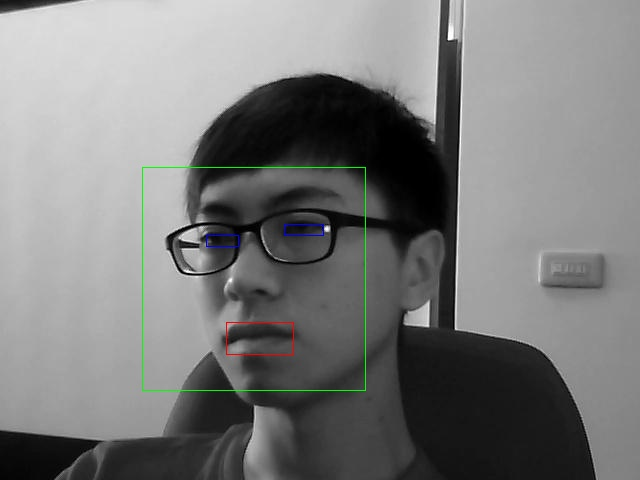
\includegraphics[
    width=0.95\linewidth,
    height=3cm,
    keepaspectratio
    ]{images/001_glasses_sleepyCombination_1002_drowsy.jpg}
}
\caption*{b) \texttt{sleepyCombination}}
\end{minipage}
\hfill
\begin{minipage}{0.28\textwidth}
\centering
\fbox{
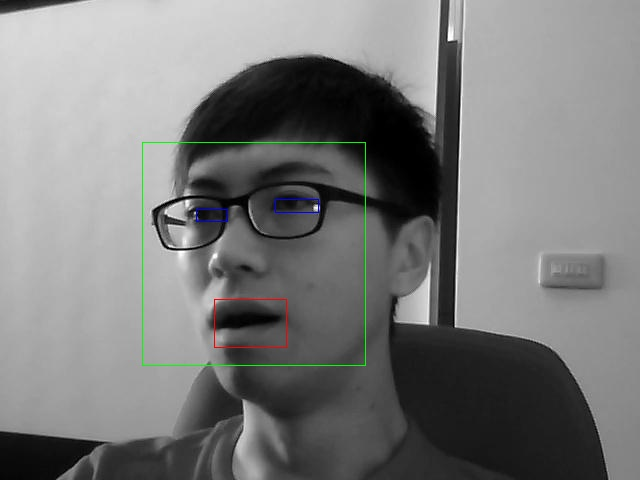
\includegraphics[
    width=0.95\linewidth,
    height=3cm,
    keepaspectratio
    ]{images/001_glasses_yawning_1001_drowsy.jpg}
}
\caption*{c) \texttt{yawning}}
\end{minipage}

\caption{Contoh 3 sampel dataset NTHU-DDD dari kelas yang berbeda}
\label{fig:contoh-dataset}

\end{figure}
\end{sloppypar}

Langkah \textit{pre-processing} yang dilakukan adalah ekstraksi \textit{bounding box} otomatis menggunakan teknik \textit{HSV Masking}. Karena posisi wajah pengemudi pada dataset ditandai dengan kotak berwarna (hijau, merah, atau biru), \textit{masking} dilakukan untuk mengambil koordinat ujung (x1, y1, x2, y2) dari kotak tersebut. Gambar kemudian diubah ukurannya (\textit{resize}) menjadi resolusi $640 \times 640$ piksel. Pembagian data dilakukan dengan proporsi 75\% untuk \textit{training}, 15\% untuk \textit{validation}, dan 10\% untuk \textit{testing}. Untuk memastikan hasil yang konsisten saat diulang, \textit{random seed} diatur pada nilai 42.

\begin{table}[h!]
\centering
\caption{Pembagian dataset}
\label{tab:split-data}
\begin{tabular}{lrr}
\toprule
\textbf{Subset} & \textbf{Jumlah Sampel} & \textbf{Rasio (\%)} \\
\midrule
Training   & 49.890 & 75\% \\
Validation & 9.978 & 15\% \\
Test       & 6.653 & 10\% \\
\midrule
\textbf{Total} & \textbf{66.521} & \textbf{100\%} \\
\bottomrule
\end{tabular}
\end{table}

\section{Konfigurasi Eksperimen}
\begin{petunjuk}
Tabel hyperparameter (learning rate, batch size, epoch, optimizer, scheduler, dropout, dst.), loss function/reward function, hardware (GPU/CPU, RAM, durasi training), framework dan versi.
\end{petunjuk}

Sistem \textit{Vision Guard} dilatih menggunakan arsitektur Faster R-CNN dengan \textit{backbone} ResNet-50 FPN dan bobot awal (\textit{pre-trained weights}) dari dataset COCO. Lingkungan eksperimen dijalankan menggunakan \textit{framework} PyTorch dan Torchvision pada Google Colab menggunakan GPU Tesla T4 (VRAM 15.6 GB). Tabel \ref{tab:hyperparam} menyajikan nilai \textit{hyperparameter} yang digunakan selama proses pembuatan model.

\begin{table}[h!]
\centering
\caption{Hyperparameter eksperimen}
\label{tab:hyperparam}
\begin{tabular}{ll}
\toprule
\textbf{Hyperparameter} & \textbf{Nilai} \\
\midrule
Arsitektur Model & Faster R-CNN (ResNet-50 FPN) \\
Learning rate    & 0.005 \\
Batch size       & 4 \\
Epoch Maksimal   & 20 \\
Optimizer        & SGD (Momentum = 0.9, Weight Decay = $5\times10^{-4}$) \\
Scheduler        & StepLR (Step Size = 7, Gamma = 0.1) \\
Score Threshold  & 0.5 \\
NMS Threshold    & 0.4 \\
Random seed      & 42 \\
\bottomrule
\end{tabular}
\end{table}

\section{Metrik Evaluasi}
\begin{petunjuk}
Pilih metrik yang \textbf{sesuai konteks} (bukan hanya akurasi). Justifikasi singkat pemilihan metrik (mis. ``F1-macro dipilih karena dataset \textit{imbalanced}'').
\end{petunjuk}

Metrik evaluasi yang digunakan adalah \textit{Mean Average Precision} (mAP) yang dihitung menggunakan pustaka \texttt{torchmetrics}. mAP dipilih karena merupakan metrik standar untuk tugas \textit{object detection}. Metrik ini mengukur akurasi klasifikasi kelas perilaku sekaligus mengukur seberapa akurat posisi \textit{bounding box} yang diprediksi dibandingkan dengan nilai asli (\textit{ground truth}) melalui perhitungan \textit{Intersection over Union} (IoU). Evaluasi difokuskan pada nilai mAP@[0.5:0.95] dan mAP@0.50.

\section{Hasil Kuantitatif}
\begin{petunjuk}
Tabel utama metrik untuk train/val/test. Bandingkan $\geq 2$ konfigurasi (mis. dengan vs tanpa \textit{augmentation}, atau model utama vs \textit{baseline}). Sertakan \textit{standard deviation} atau \textit{confidence interval} bila menjalankan multiple seed.
\end{petunjuk}

Eksperimen menunjukkan bahwa proses \textit{training} model berjalan dengan baik. Evaluasi dilakukan pada setiap \textit{epoch} terhadap \textit{validation set}. Model terbaik didapatkan pada Epoch ke-3 dengan nilai mAP \textit{validation} sebesar 0.8785. Ketika model terbaik ini diuji menggunakan \textit{Test Set} (6.653 gambar), model menghasilkan nilai mAP@0.5:0.95 sebesar 0.8749 dan mAP@0.50 sebesar 0.9343.

\begin{table}[h!]
\centering
\caption{Hasil kuantitatif model (Metrik: mAP@0.5:0.95)}
\label{tab:hasil}
\begin{tabular}{lcc}
\toprule
\textbf{Konfigurasi} & \textbf{Validation} & \textbf{Test} \\
\midrule
Epoch 1     & 0.8148 & - \\
Epoch 2     & 0.8070 & - \\
\textbf{Epoch 3 (Best Model)} & \textbf{0.8785} & \textbf{0.8749} \\
Epoch 4     & 0.8425 & - \\
Epoch 5     & 0.8714 & - \\
\bottomrule
\end{tabular}
\end{table}

Jika dilihat berdasarkan performa per kelas pada \textit{Test Set}, kelas \texttt{sleepyCombination} mendapatkan skor mAP tertinggi sebesar 0.9175, diikuti oleh \texttt{yawning} (0.8680), \texttt{slowBlinkWithNodding} (0.8572), dan \texttt{notdrowsy} (0.8568).

\section{Analisis \textit{Hyperparameter Tuning}}
\begin{petunjuk}
Dokumentasi proses tuning (\textit{grid/random/Bayesian search}). Sertakan grafik metrik vs hyperparameter kunci. Diskusikan hyperparameter mana yang paling sensitif.
\end{petunjuk}

Meskipun tidak dilakukan pencarian kombinasi parameter secara luas, pengaturan \textit{learning rate scheduling} (\texttt{StepLR}) dan batas \textit{Non-Maximum Suppression} (NMS) terbukti sangat penting. Nilai \textit{NMS Threshold} sebesar 0.4 diatur agar kotak prediksi pada area wajah pengemudi tidak menumpuk secara berlebihan. Penggunaan bobot \textit{pre-trained} COCO membantu model untuk mengenali fitur dasar gambar dengan cepat, sehingga model sudah mencapai mAP yang optimal pada Epoch ke-3 sebelum akhirnya mengalami fluktuasi nilai yang stabil pada epoch berikutnya.

\section{Hasil Kualitatif \& \textit{Error Analysis}}
\begin{petunjuk}
Contoh prediksi benar \& salah (minimal 3 kasus salah). \textit{Confusion matrix} atau contoh prediksi vs \textit{ground truth} atau \textit{reward curve}. Hipotesis penyebab kegagalan + mitigasi yang dicoba.
\end{petunjuk}

Secara kualitatif, model mampu mendeteksi letak wajah pengemudi serta mengklasifikasikan ekspresi \textit{yawning} dan \textit{sleepyCombination} dengan akurat karena adanya fitur visual yang jelas seperti bentuk mulut terbuka atau posisi kepala. Namun, terdapat beberapa jenis kesalahan (\textit{error}) yang ditemukan:
\begin{enumerate}
    \item \textbf{Kesalahan deteksi antara \textit{Not Drowsy} dan \textit{Slow Blink}:} Gambar pada kelas \texttt{notdrowsy} terkadang diprediksi sebagai \texttt{slowBlinkWithNodding}. Hal ini terjadi karena gerakan kedipan mata normal yang tidak sengaja terekam pada satu frame tunggal dianggap oleh model sebagai kondisi mata tertutup akibat mengantuk.
    \item \textbf{\textit{False Positives} pada pencahayaan yang kurang:} Pada beberapa kondisi gambar yang gelap, objek di latar belakang yang memiliki warna atau tekstur mirip kulit wajah terkadang ikut terdeteksi secara keliru.
\end{enumerate}
Sebagai langkah perbaikan, penggunaan arsitektur yang mendukung pengolahan data runtun waktu (\textit{temporal}) seperti gabungan CNN dengan LSTM dapat dipertimbangkan agar sistem bisa membedakan durasi kedipan mata biasa dengan kedipan akibat kantuk.

\section{Pembahasan}
\begin{petunjuk}
Interpretasi hasil terhadap rumusan masalah Bab I. Perbandingan dengan literatur (lebih baik / setara / lebih buruk → mengapa?). Keterbatasan eksperimen.
\end{petunjuk}

Hasil eksperimen ini menjawab rumusan masalah mengenai kemampuan arsitektur Faster R-CNN dalam mendeteksi tingkat kelelahan pengemudi. Dengan nilai mAP pengujian yang mencapai 0.8749 dan mAP@0.50 sebesar 0.9343, model Faster R-CNN terbukti sangat baik dalam menentukan posisi dan mengelompokkan ekspresi wajah dari data gambar dua dimensi.

Jika dibandingkan dengan metode deteksi tradisional, pendekatan berbasis \textit{deep learning} pada \textit{Vision Guard} ini jauh lebih tangguh menghadapi variasi posisi wajah. Keterbatasan utama dari eksperimen ini adalah model hanya bekerja pada frame gambar mandiri (fitur spasial 2D) sehingga tidak dapat melihat durasi dari suatu gerakan (fitur temporal). Meskipun demikian, performa deteksi yang dihasilkan sudah sangat memadai untuk menjadi dasar pengembangan sistem keselamatan berkendara.

%==============================================================================
% BAB IV - PEMBAGIAN TUGAS & DEKLARASI KONTRIBUSI INDIVIDUAL
%==============================================================================
\chapter{PEMBAGIAN TUGAS \& DEKLARASI KONTRIBUSI INDIVIDUAL}
\label{bab:kontribusi}

\begin{petunjuk}
\textbf{BAB INI WAJIB DITULIS SECARA MANDIRI OLEH MASING-MASING ANGGOTA} (bukan oleh ketua kelompok). Isi Sub-bab ini akan digunakan untuk men-generate pertanyaan ujian lisan yang personal. Klaim penguasaan konsep per anggota dideklarasikan dalam berkas \texttt{metadata.json} (field \texttt{konsep\_dikuasai\_*}) yang merupakan bagian tidak terpisahkan dari laporan ini.

Gandakan template di bawah untuk setiap anggota (3--4 orang).
\end{petunjuk}

\section{Benedict Aurelius -- NPM. 2306209095}

\subsection*{IV.1.1 Komponen yang Dikerjakan}
Daftar konkret bagian proyek yang menjadi tanggung jawab penuh saya:
\begin{itemize}[leftmargin=*]
    \item \textbf{Kode/modul:} Menyusun \textit{training loop} utama pada PyTorch, mengonfigurasi \textit{optimizer} (SGD), dan mengimplementasikan \textit{learning rate scheduler} (\texttt{StepLR}).
    \item \textbf{Bagian arsitektur:} Inisialisasi arsitektur Faster R-CNN dengan \textit{backbone} ResNet-50 FPN, memuat \textit{pre-trained weights} COCO, serta menyesuaikan \textit{classifier head} untuk 4 kelas target.
    \item \textbf{Bagian analisis:} Analisis konvergensi \textit{loss} selama proses \textit{training} dan eksperimen \textit{hyperparameter tuning} untuk menentukan \textit{epoch} yang optimal.
    \item \textbf{Bagian laporan:} Menyusun Bab II (Pendekatan AI) khususnya bagian landasan teori dan justifikasi ilmiah arsitektur.
\end{itemize}

\subsection*{IV.1.2 Pernyataan Penggunaan AI \textit{Assistant}}
\begin{itemize}[leftmargin=*]
    \item \textbf{Tool yang dipakai:} Gemini.
    \item \textbf{Untuk bagian apa:} \textit{Debugging} kode PyTorch/framework saat proses \textit{training} dan pemecahan \textit{error}, serta \textit{review} dokumentasi teknis Faster R-CNN.
    \item \textbf{Tingkat ketergantungan:} Rendah - Sedang (estimasi $\sim$20\% output berasal dari AI).
    \item \textbf{Pernyataan:} Saya memahami dan dapat mempertanggungjawabkan setiap baris kode/teks yang saya klaim sebagai bagian saya.
\end{itemize}

%-------------------- Anggota 2 ---------------------------------------------
\section{Deandro Najwan Ahmad Syahbanna -- NPM. 2306213174}

\subsection*{IV.2.1 Komponen yang Dikerjakan}
Daftar konkret bagian proyek yang menjadi tanggung jawab penuh saya:
\begin{itemize}[leftmargin=*]
    \item \textbf{Kode/modul:} Mengembangkan skrip pra-pemrosesan data, termasuk otomatisasi ekstraksi \textit{bounding box} menggunakan algoritma \textit{HSV Masking} dari gambar mentah.
    \item \textbf{Bagian arsitektur:} Membuat \textit{custom dataset pipeline} pada PyTorch (Dataloader) agar gambar dan anotasi \textit{bounding box} dapat diproses oleh model dalam format \textit{batch}.
    \item \textbf{Bagian analisis:} Menganalisis distribusi kelas pada dataset NTHU-DDD dan memastikan pembagian subset \textit{training, validation,} dan \textit{testing} berjalan proporsional (75:15:10).
    \item \textbf{Bagian laporan:} Menulis draf utama untuk Bab I (Pendahuluan) dan Bab V (Kesimpulan \& Pekerjaan Lanjutan).
\end{itemize}

\subsection*{IV.2.2 Pernyataan Penggunaan AI \textit{Assistant}}
\begin{itemize}[leftmargin=*]
    \item \textbf{Tool yang dipakai:} Gemini.
    \item \textbf{Untuk bagian apa:} Pencarian referensi teori pendekatan AI, perbaikan struktur \textit{object detection pipeline}, dan \textit{formatting} dokumen.
    \item \textbf{Tingkat ketergantungan:} Rendah (estimasi $\sim$20\% output berasal dari AI).
    \item \textbf{Pernyataan:} Saya memahami dan dapat mempertanggungjawabkan setiap baris kode/teks yang saya klaim sebagai bagian saya.
\end{itemize}

%-------------------- Anggota 3 ---------------------------------------------
\section{Nelson Laurensius -- NPM. 2306161845}

\subsection*{IV.3.1 Komponen yang Dikerjakan}
Daftar konkret bagian proyek yang menjadi tanggung jawab penuh saya:
\begin{itemize}[leftmargin=*]
    \item \textbf{Kode/modul:} Mengimplementasikan skrip evaluasi metrik menggunakan pustaka \texttt{torchmetrics} untuk menghitung nilai \textit{Mean Average Precision} (mAP).
    \item \textbf{Bagian arsitektur:} Mengembangkan pipa otomatisasi pemrosesan JSON untuk menghasilkan dokumen \textit{metadata} proyek yang terstruktur.
    \item \textbf{Bagian analisis:} Mengumpulkan hasil evaluasi kuantitatif (mAP@[0.5:0.95] dan mAP@0.50) dan membandingkan kinerja model antar setiap \textit{epoch}.
    \item \textbf{Bagian laporan:} Menyusun berkas \texttt{metadata.json} (Lampiran A) secara utuh dan memformat referensi daftar pustaka.
\end{itemize}

\subsection*{IV.3.2 Pernyataan Penggunaan AI \textit{Assistant}}
\begin{itemize}[leftmargin=*]
    \item \textbf{Tool yang dipakai:} Gemini.
    \item \textbf{Untuk bagian apa:} Bantuan penyusunan struktur \textit{metadata} (JSON) proyek , \textit{debugging environment} NumPy saat evaluasi metrik, dan \textit{formatting} kode LaTeX.
    \item \textbf{Tingkat ketergantungan:} Rendah (estimasi $\sim$20\% output berasal dari AI).
    \item \textbf{Pernyataan:} Saya memahami dan dapat mempertanggungjawabkan setiap baris kode/teks yang saya klaim sebagai bagian saya.
\end{itemize}

%-------------------- Anggota 4 ---------------------------------------------
\section{Wesley Frederick Oh -- NPM. 2306202763}

\subsection*{IV.4.1 Komponen yang Dikerjakan}
Daftar konkret bagian proyek yang menjadi tanggung jawab penuh saya:
\begin{itemize}[leftmargin=*]
    \item \textbf{Kode/modul:} Menulis skrip \textit{inference} untuk pengujian model dan visualisasi hasil akhir, termasuk fungsi untuk menggambar \textit{bounding box} beserta label pada gambar \textit{Test Set}.
    \item \textbf{Bagian arsitektur:} Mengkalibrasi parameter pada tahap \textit{post-processing}, secara spesifik menyesuaikan \textit{Non-Maximum Suppression} (NMS) \textit{threshold} di angka 0.4 untuk mencegah deteksi ganda pada area wajah.
    \item \textbf{Bagian analisis:} Melakukan analisis kualitatif dan \textit{error analysis} untuk mengidentifikasi penyebab klasifikasi yang salah (\textit{false positives} dan masalah pencahayaan).
    \item \textbf{Bagian laporan:} Menulis seluruh Bab III (Implementasi \& Hasil Eksperimen), Bab IV (Pembagian Tugas), serta mengatur format kompilasi akhir LaTeX.
\end{itemize}

\subsection*{IV.4.2 Pernyataan Penggunaan AI \textit{Assistant}}
\begin{itemize}[leftmargin=*]
    \item \textbf{Tool yang dipakai:} Gemini.
    \item \textbf{Untuk bagian apa:} Bantuan penyusunan draf narasi latar belakang dan perbaikan tata bahasa, serta \textit{formatting} struktur laporan akhir menggunakan LaTeX.
    \item \textbf{Tingkat ketergantungan:} Rendah (estimasi $\sim$20\% output berasal dari AI).
    \item \textbf{Pernyataan:} Saya memahami dan dapat mempertanggungjawabkan setiap baris kode/teks yang saya klaim sebagai bagian saya.
\end{itemize}

%==============================================================================
% BAB V - KESIMPULAN & PEKERJAAN LANJUTAN
%==============================================================================
\chapter{KESIMPULAN \& PEKERJAAN LANJUTAN}
\label{bab:kesimpulan}

\section{Kesimpulan}
\begin{petunjuk}
3--5 poin yang \textbf{menjawab langsung} rumusan masalah Bab I. Sertakan angka konkret (bukan klaim umum seperti ``model bekerja dengan baik''). Setiap poin dapat ditelusuri ke seksi tertentu di Bab III.
\end{petunjuk}

\begin{enumerate}[leftmargin=*]
    \item {[Kesimpulan terhadap RM1]}
    \item {[Kesimpulan terhadap RM2]}
    \item {[Kesimpulan terhadap RM3]}
\end{enumerate}

\section{Klaim Bonus Skor}
\begin{petunjuk}
Centang yang relevan; hapus seksi ini jika tidak mengklaim bonus.
\end{petunjuk}

\begin{itemize}[leftmargin=*]
    \item[$\square$] \textbf{B1. Evaluasi Komparatif \& Iterasi} → bukti pada Subbab 3.4 dan 3.5
    \item[$\square$] \textbf{B2. Dataset Mandiri} → bukti pada Subbab 3.1 + Lampiran B
    \item[$\square$] \textbf{B3. Analisis Etika, Bias, \& Keterbatasan} → bukti pada Subbab 3.7
\end{itemize}

\section{Pekerjaan Lanjutan (\textit{Future Work})}
\begin{petunjuk}
3--5 arah pengembangan yang \textbf{spesifik dan realistis} (bukan ``meningkatkan akurasi''). Mis. ``mengevaluasi pada dataset out-of-domain X'', ``mengganti backbone dengan ViT-B/16'', ``menambahkan modul interpretability Grad-CAM''.
\end{petunjuk}

\begin{enumerate}[leftmargin=*]
    \item {[Arah pengembangan pertama]}
    \item {[Arah pengembangan kedua]}
\end{enumerate}

%==============================================================================
% DAFTAR PUSTAKA
%==============================================================================
\printbibliography[heading=bibintoc,title={DAFTAR PUSTAKA}]

%==============================================================================
% LAMPIRAN
%==============================================================================
\appendix
\renewcommand{\thechapter}{\Alph{chapter}}
\titleformat{\chapter}[display]
  {\normalfont\Large\bfseries\centering}
  {\appendixname\ \thechapter}{12pt}{\Large}

%------ Lampiran A: Metadata JSON --------------------------------------------
\chapter{Berkas Metadata Proyek (JSON)}
\label{lamp:metadata}

\begin{petunjuk}
Tempelkan isi berkas \texttt{metadata.json} yang juga dikumpulkan terpisah. Berkas ini diumpan ke sistem agentic AI untuk men-generate pertanyaan ujian lisan. Ikuti skema pada \texttt{Template Metadata Proyek (JSON).md}.
\end{petunjuk}

\begin{lstlisting}[language=json]
{
  "kode_kelompok": "K00",
  "topik_pilihan": 0,
  "judul_proyek": "...",
  "anggota": [
    {
      "nama": "...",
      "npm": "...",
      "konsep_dikuasai_implementasi": ["..."],
      "konsep_dikuasai_teori": ["..."]
    }
  ]
}
\end{lstlisting}

%------ Lampiran B: Tautan Repositori & Dataset ------------------------------
\chapter{Tautan Repositori \& Dataset}
\label{lamp:tautan}

\begin{description}[leftmargin=4cm,labelwidth=3.5cm]
    \item[GitHub repo:] \url{https://github.com/...}
    \item[Google Colab:] \url{https://colab.research.google.com/...}
    \item[Dataset mandiri:] \url{...} (jika ada; isi ``--'' jika tidak)
    \item[Video demo:] \url{...} (opsional)
\end{description}

\textbf{Status akses:} repositori publik / Colab dengan permission ``anyone with the link can view''. Sudah diverifikasi terbuka pada [tanggal].

%------ Appendix C: Research Participation Consent Form (Informed Consent) ---
% Section in English (rest of the report remains in Bahasa Indonesia).
\renewcommand{\appendixname}{APPENDIX}

\chapter{Research Participation Consent Form (\textit{Informed Consent})}
\label{lamp:consent}

\begin{petunjuk}
\small
\textbf{REQUIRED} to be signed by each group member before report submission. Declining participation (Option C) does not affect academic grades.
\end{petunjuk}

{\small
\textbf{C.1\quad Brief Explanation.}
\textit{Research:} Development \& validation of an \textit{agentic AI} framework for supporting academic oral examinations.
\textit{Principal investigator:} [Name of course lecturer], Department of Computer Engineering, Universitas Indonesia. \textit{Co-investigator:} a final-year undergraduate student supervised by the principal investigator.
\textit{Contact:} \texttt{[principal investigator's email]}. \textit{Ethics review status:} \textbf{under review}.
\textit{Context:} data collection is conducted alongside the oral examination of the AI course's final assessment. The oral examination is held as part of the academic assessment regardless of the participant's research-participation choice.

\textbf{C.2\quad Data Collected.}
Final report (PDF) and \texttt{metadata.json} file; audio and video recordings of the oral examination; automatic transcripts derived from those recordings; lecturer's \textit{judgment} scores (\textit{ground truth}) and AI system's \textit{judgment} scores (test variable). \textbf{Not collected:} biometric data other than voice/face, or personal data beyond what is contained in the academic report.

\textbf{C.3\quad Data Management.}
\textbf{Participant names and student IDs (NPMs) will be stored anonymously} --- replaced with participant codes (\texttt{P001}, \texttt{P002}, \ldots) prior to analysis. The code-to-identity mapping table is stored separately, encrypted, and accessed only by the principal investigator. Publications (journal articles, conference papers, theses) will not contain individual identities. Data is stored with encryption on infrastructure managed by the research team; retention is 5 years after the research concludes, after which the data is permanently deleted. Access is limited to the principal and co-investigators; no third party may access without an amendment to this \textit{consent}.

\textbf{C.4\quad Participant Rights.}
(1)~The right to decline participation without affecting the course grade. (2)~The right to partial participation (e.g.\ report/metadata may be used, video recording may not). (3)~The right to withdraw data at any time \textbf{until 30 June 2026} by emailing the principal investigator with the subject \texttt{[Withdrawal] - [Name] - [NPM]}; confirmation of deletion is provided within $\le$~7 working days. After 30 June 2026 the data will have entered the analysis phase and withdrawal becomes impractical. (4)~The right to ask questions at any time to the principal investigator. (5)~The right to receive a summary of the research findings once they are published (sent to the registered email).

\textbf{C.5\quad Individual Consent.}
Each member completes their personal block on the following pages --- one page per member. Tick \textbf{exactly one} of the three options (A / B / C), then sign with a wet signature or an \textit{e-signature}.
}

%----------------------------------------------------------------------------
% PER MEMBER — one page each
%----------------------------------------------------------------------------
\newcommand{\memberBlock}[1]{%
\newpage
\section*{Individual Consent --- Member #1}

\noindent
\begin{tabular}{p{0.28\textwidth}p{0.65\textwidth}}
Full name        & : [Name of Member #1] \\
Student ID (NPM) & : [xxxxxxxxxx] \\
Email            & : [\ldots] \\
\end{tabular}

\vspace{1.5em}

I have read Sections C.1--C.4 and understood their contents. I voluntarily choose the following option:

\vspace{0.5em}

\begin{itemize}[leftmargin=2em, label={$\square$}, itemsep=0.8em]
    \item \textbf{Option A --- Full Participation.} I consent to the use of my report, metadata, \textbf{and} the audio and video recordings of my oral examination for research purposes.
    \item \textbf{Option B --- Limited Participation.} I consent to the use of my report, metadata, and audio recording, \textbf{but I do not consent to the video recording} of my oral examination being used for research. (The video recording will be deleted after the academic assessment is completed.)
    \item \textbf{Option C --- Decline Participation.} I decline to participate in the research. (The academic oral examination proceeds as usual; there is no consequence to the grade.)
\end{itemize}

\vfill

\noindent
\begin{tabular}{p{0.45\textwidth}p{0.45\textwidth}}
\centering Participant's signature & \centering Witness / researcher's signature \tabularnewline[2.5cm]
\centering (\hspace{4cm}) & \centering (\hspace{4cm}) \tabularnewline
\centering Date: \hspace{3cm} & \centering Date: \hspace{3cm} \tabularnewline
\end{tabular}

\vspace{1em}
}

\memberBlock{1}
\memberBlock{2}
\memberBlock{3}
\memberBlock{4}

\end{document}
